\documentclass[a4paper,11pt]{article}
\usepackage[polish]{babel}
\usepackage[T1]{fontenc}
\usepackage[utf8]{inputenc}
\usepackage{listings}
\usepackage{multicol}
\usepackage{comment}
\usepackage{adjustbox}
\usepackage{amsfonts}
\usepackage{amsmath}
\usepackage{amssymb}
\usepackage{bbm}
\usepackage{latexsym}
\usepackage{wasysym}
\usepackage{amsthm}
\usepackage{indentfirst}
\usepackage{setspace}
\usepackage{array}
\usepackage{multirow}
\usepackage{geometry}
\usepackage{hyperref}
%\usepackage{gensymb}
\usepackage{algorithm}
\usepackage{algpseudocode,amsmath}
\usepackage{tikz} % do grafów
\usepackage[inkscapeformat=png]{svg}
\geometry{hdivide={2cm,*,2cm}}
\geometry{vdivide={2cm,*,2cm}}
\usepackage{microtype}

\usepackage{changepage}
\usepackage{array,booktabs}

\newcommand{\var}{\texttt}

\graphicspath{{images/}}

%\usepackage{titlesec}
%\titlespacing{\section}{0ex}{1ex}{1ex} % zmniejszenie odstępów przed i po tytule rozdziału...
%\titleformat*{\section}{\sf\large\bfseries} % i zmiana kroju czcionki
%\titlespacing{\subsection}{0ex}{0.75ex}{0.75ex} % % j/w dla tytułów podrozdziałów
%\titleformat*{\subsection}{\sf\bfseries}

\usepackage{enumitem}
\setlist{
	itemsep=0pt,
	parsep=2pt,
	topsep=5pt,
	leftmargin=15pt	
}

\usepackage{caption, sidecap}
\usepackage{subcaption}
\captionsetup{
	font=footnotesize,
	skip=0pt,
}
%\setlength{\captionmargin}{3ex}

\usepackage{graphicx, wrapfig, float}
\usepackage{epstopdf}
%\usepackage{subfig}

% Zmniejszenie odstępów przed i za wzorami wystawionymi
%\AtBeginDocument
%{
%\addtolength{\abovedisplayskip}{-1ex}
%\addtolength{\abovedisplayshortskip}{-1ex}
%\addtolength{\belowdisplayskip}{-1ex}
%\addtolength{\belowdisplayshortskip}{-1ex}
%}

\usepackage{titlesec}
\titlelabel{\thetitle.\quad}

%\textheight 24 cm
%\textwidth 16 cm
%\hoffset = -1.5 cm
\voffset = -0.3 cm

\usepackage{fancyhdr}
\usepackage{layout}
\usepackage{setspace}

%\def\tablename{Tabela} % bez tej linii nazwą tabeli byłaby "Tablica"

\usepackage{siunitx}[=v2]

\renewcommand{\baselinestretch}{1}
\setlength{\headheight}{0pt}


\setlength{\headheight}{0pt}
\title{\vspace{5ex}\Huge\textbf{AutoML} \\ 
\LARGE{\vspace{2ex}Tunowalność algorytmów i hiperparametrów}\vspace{10ex}}
\author{
		Bartosz Kaczorowski \vspace{1ex}\\
        Damian Kąkol \vspace{1ex}\\
        Jakub Kępka 
        \vspace{3ex}
}
\date{\vspace{50ex} Listopad 2024}

%\setlength\parindent{0pt}

\begin{document}
\doublespacing{}

% strona tytułowa
\clearpage\maketitle
\thispagestyle{empty}

% tutaj stopka
\pagestyle{fancy}
\fancyhf{}
\fancyfoot[c]{Wydział Matematyki i Nauk Informacyjnych Politechniki Warszawskiej}
\fancyfoot[r]{\thepage}
\footskip=30pt

\renewcommand{\footruleskip}{10pt}
\renewcommand{\headrulewidth}{0pt}
\renewcommand{\footrulewidth}{1pt}

\newpage
\tableofcontents
\onehalfspacing{}

\newpage
\section{Wstęp}
Celem niniejszego raportu jest analiza tunowalności hiperparametrów trzech wybranych algorytmów uczenia maszynowego (Elastic Net, XGBoost, Random Forest) na czterech zbiorach danych. Analiza obejmie wykorzystanie dwóch różnych metod doboru punktów (tzw. \textit{samplingu}) w procesie optymalizacji hiperparametrów:
\begin{itemize}
    \item przeszukiwanie losowe - ang. \textit{Random Search}\cite{RS},
    \item optymalizację bayesowską - ang. \textit{Bayes Optimization}\cite{BS}.
\end{itemize}

W pracy zostanie przeanalizowana liczba iteracji każdej metody potrzebna, aby uzyskać stabilne wyniki, różnica w tunowalności między różnymi algorytmami oraz to, czy i jak dana technika doboru punktów wpływa na wyniki i wnioski dotyczące tunowalności.

Bieżący raport bazowany jest na pracy \textit{"Tunability: Importance of Hyperparameters of Machine Learning Algorithms"}\cite{tuna}, gdzie została opisana między innymi tunowalność algorytmów i ich hiperparametrów.

\section{Dane}
\label{sec:data}
Optymalizaja algorytmów i ich hiperparametrów została wykonana na czterech zbiorach danych dostępnych na platformie \textit{OpenML}, każdy z nich dotyczy problemu klasyfikacji binarnej:
\begin{itemize}
    \item \textbf{credit-g} (1000 instancji, 21 cech) - klasyfikacja osób na te o dobrej lub złej zdolności kredytowej;
    \item \textbf{diabetes} (768 instancji, 9 cech) - ocena czy dany pacjent wykazuje objawy cukrzycy zgodnie z kryteriami WHO. Badana populacja obejmuje osoby zamieszkałe w Phoenix, Arizona, USA;
    \item \textbf{spambase} (4601 instancji, 58 cech) - klasyfikacja e-maili na bazie treści, określająca czy są spamem. Kolekcja e-maili oznaczonych jako spam pochodziła od administratora poczty oraz osób zgłaszających spam, natomiast wiadomości niespamowe były zbierane z poczty służbowej i osobistej;
    \item \textbf{yeast} (2417 instancji, 117 cech) - zbiór danych dotyczący drożdży (opisany przez Elisseeffa i Westona, 2002), zawiera dane z mikro-macierzy ekspresji genów oraz profile filogenetyczne drożdży. W sumie gen może mieć przypisanych 14 różnych etykiet ze względu na 7 różnych, binarnych klas - na potrzeby naszej analizy wykorzystano tylko klasę o nazwie \texttt{Class1}.
\end{itemize}

\section{Tunowalność algorytmów i hiperparametrów}
Przed przejściem do analizy tunowalności, należy przytoczyć kilka definicji z artykułu\cite{tuna} wspomnianym na wstępie.

Najlepszą konfiguracją hiperparametrów dla zbioru danych $j$ nazywać będziemy wektor:
\begin{equation}
    \label{best_params}
    \theta^{(j)*} := \arg \min_{\theta \in \Theta} R^{(j)}(\theta).
\end{equation}

Do oceny tunowalności algorytmów i ich hiperparametrów niezbędny będzie zestaw optymalnych hiperparametrów (zwanych też \textit{defaultowymi}) dla $m$ zbiorów danych, zdefiniowany w następujący sposób:
\begin{equation}
    \label{default_params}
    \theta^* := \arg \min_{\theta \in \Theta} g\left(R^{(1)}(\theta), \ldots, R^{(m)}(\theta)\right).
\end{equation}

W definicjach \eqref{best_params} i \eqref{default_params} $R^{(j)}(\theta)$ oznacza metrykę mierzącą poprawność alogorytmu (dobrą miarą będzie tu -AUC \cite{AUC}), zaś $g$ oznacza funkcję agregującą, np. średnią. To czy miara $R^{(j)}(\theta)$ powinna być znormalizowana przed zagregowaniem, będzie przedmiotem analizy zawartej w dalszych rozdziałach.

Do mierzenia tunowalności algorytmu na zbiorze danych $j$ wykorzystana zostanie miara określona w sposób następujący:
\begin{equation}
    \label{alg_tun}
    d^{(j)} := R^{(j)}(\theta^*) - R^{(j)}(\theta^{(j)*}), \quad \text{dla } j = 1, \ldots, m.
\end{equation}

Podobnie jak w \eqref{alg_tun}, by móc zmierzyć tunowalności pojedynczego $i$-tego hiperparametru definiujemy:
\begin{equation}
    \label{hyp_tun}
    d^{(j)}_i := R^{(j)}(\theta^*) - R^{(j)}(\theta^{(j)*}_i), \quad \text{dla } j = 1, \ldots, m, 
\end{equation}
gdzie $\theta^{(j)*}_i$ oznacza najlepszą wartości hiperparametru na zbiorze danych $j$ (podczas gdy pozostałe parametry pochodzą z optymalnego zestawu $\theta^*$), zgodnie ze wzorem:
\begin{equation*}
    \theta^{(j)*}_i := \arg \min_{\theta \in \Theta, \theta_l = \theta^*_l \, \forall l \neq i} R^{(j)}(\theta)
\end{equation*}
Metryki \eqref{alg_tun} i \eqref{hyp_tun} można następnie zagregować pomiędzy zbiorami poprzez wyliczenie średniej lub mediany opisanej różnicy, w celu uzyskania szerszego obrazu przeprowadzonych optymalizacji.

Ostatnią przydatną miarą może okazać się jeszcze względna tunowalność $i$-tego hiperparametru względem algorytmu na zbiorze $j$ :
\begin{equation}
    \label{wzg_tun}
    d^{(j), \text{rel}}_i = \frac{d^{(j)}_i}{d^{(j)}}
\end{equation}

\subsection{Elastic Net}
\label{sec:elnet}
Do zaimplementownania modelu \textit{Elastic Net}\cite{elnet} wykorzystano klasę \texttt{LogisticRegression} z pakietu \textit{scikit-learn} z parametrem \texttt{penalty} ustawionym na \texttt{elasticnet} oraz \texttt{solver} na \texttt{saga}. Z innych istotnych hiperparametrów, przyjęto liczbę 200 jako maksymalną liczbę iteracji, a także ustawiono \texttt{class\_weight} na \texttt{balanced} w celu wyrównania nierówności związanych z dysproporcjami klas.

Do przeszukiwania losowego zastosowano klasę \texttt{RandomizedSearchCV} z tego samego pakietu, zaś do optymalizacji bayesowskiej klasę \texttt{BayesSearchCV} z pakietu \textit{scikit-optimize}. Obie metody wykorzystywały do pomiaru metrykę \texttt{roc\_auc}, a także kroswalidację (ustawioną na 5). Co istotne, w obu przypadkach ustawiono ten sam \texttt{random\_state}, dzięki temu metody korzystały z tej samej siatki hiperparametrów. Przeszukiwanie losowe w trakcie optymalizacji wykonywało 180 iteracji - optymalizacja bayesowska zaś 3 razy mniej.

\paragraph{Określenie przestrzeni hiperparametrów i optymalnego zestawu \vspace{2ex} \\}

Model \textit{Elastic Net} posiada dwa główne hiperparametry, ich zakresy zaczerpnięto z artykułu\cite{tuna}:
\begin{itemize}
    \item \textbf{C} - rozkład logarytmiczno-jednostajny od $2^{-10}$ do $2^{10}$,
    \item \textbf{l1\_ratio} - rozkład jednostajny od 0 do 1.
\end{itemize}

Do określenia optymalnego zestawu hiperparametrów wykorzystano przeszukiwanie losowe. Za funkcję $g$ z definicji \eqref{default_params} przyjęto średnią, zaś $R^{(j)}(\theta)$ rozpatrzono na trzy sposoby - przyjmując zwykłe \textit{-AUC}, znormalizowane i ustandaryzowane, co można zobaczyć na rysunku \ref{fig:elnet:auc}. Pierwsze dwa podejścia wskazały na ten sam zestaw hiperparametrów, który w toku dalszego postępowania okazał się być lepszy (wykazywał mniejsze tunability według \eqref{alg_tun} i \eqref{hyp_tun}).

\paragraph{Wyniki \vspace{2ex} \\}
 Uzyskane wyniki tunowalności algorytmu oraz jego hiperparametrów zawarte w tabeli \ref{tab:elnet:wyn} pokazują, że zysk nie jest duży, zwłaszcza w kontekście tunowalności parametru \texttt{C}, co dobrze widać patrząc na względną tunowalności w tabeli \ref{tab:elnet:rel}. Dużo większą (nawet o kilka rzędów wielkości) tunowalność zaobserwować można dla parametru \texttt{l1}, czy wogóle całego zestawu. Niemniej, zarówno średnia jak i mediana obliczanej różnicy różni się dopiero na trzecim miejscu po przecinku.

 Jeśli chodzi o różnice między samymi metodami \textit{samplingu}, to trudno określić tu jednoznacznie zwycięzcę. To co napewno można stwierdzić, to znacznie dłuższy czas iteracji optymalizacji bayesowskiej, która w skrajnym przypadku trwała średnio nawet 11 razy dłużej niż iteracja przeszukiwania losowego. To jak liczba iteracji przekłada się na wynik zostało przeanalizowane w sekcji \ref{sec:bias}.
 
\subsection{XGBoost}
Model \textit{XGBoost} był uruchamiany na 250 iteracjach dla metody \textit{Random Search} oraz 20 dla \textit{Bayes Optimization}.

\paragraph{Siatka parametrów \vspace{2ex} \\}
Zakres hiperparametrów do treningu był inspirowany artykułem do projektu. Odrzucone zostały parametry \texttt{eta}, \texttt{lambda} i \texttt{alpha} w celu przyśpieszenia procesowania, odrzucony został również dyskretny parametr \texttt{booster}. 

\paragraph{Tunowalność algorytmu \vspace{2ex} \\}
Ogólnie rzecz biorąc \textit{Random Search} częściej oferuje poprawe wydajności modelu niż optymalizacja bayesowska. Należy jednak zauważyć, że najwyższy wynik tunowalności osiągnęła optymalizacja bayesowska - około 0.0234.

\paragraph{Tunowalność hiperparametrów \vspace{2ex} \\}
Tunowalnośc poszczególnych hiperparametrów (tabela \ref{tab:xg:tunability_bayes}) wskazuje, że największe znaczenie mają parametry \texttt{subsample} i \texttt{min\_child\_weight}, które osiągają największe przyrosty efektywności na przestrzeni różnych zbiorów danych. 

\paragraph{Optymalne zakresy hiperparametrów \vspace{2ex} \\}
Analiza kwantyli dla siatki hiperparametrów (tabela \ref{tab:xg:hyperparam_grid_kwantyle}) sugeruje, że siatka startowa mogła zostać lepiej przygotowana, ponieważ niektóre kwantyle (np. \texttt{model\_\_n\_estimators}) wskazują (swoją niesymetrycznością), że górne ograniczenie mogłoby być większe.

\subsection{Random Forest}
W pracy wykorzystano algorytm \texttt{RandomForestClassifier}, który został zoptymalizowany przy użyciu technik \emph{Random Search} oraz \emph{Bayesian Optimization}. W obu metodach przyjęto określony zakres parametrów, który pozwolił na dokładne dostrojenie modelu. W \texttt{RandomizedSearchCV} ustawiono liczbę iteracji na 250 oraz w \texttt{BayesSearchCV} ustawiono liczbę iteracji na 60.\\

Zakres liczby drzew w lesie \texttt{n\_estimators} ustalono od 200 do 1740, co pozwalało na balans między dokładnością modelu a czasem jego trenowania. Głębokość każdego drzewa \texttt{max\_depth} ograniczono w przedziale od 5 do 30, aby zapobiec przetrenowaniu modelu, a jednocześnie umożliwić mu uchwycenie istotnych wzorców w danych. Minimalna liczba próbek wymagana do podziału w węźle \texttt{min\_samples\_split} została określona na przedział od 2 do 20, aby zapewnić elastyczność w tworzeniu nowych podziałów. Minimalną liczbę próbek w liściu drzewa \texttt{min\_samples\_leaf} przyjęto od 1 do 10, co chroniło przed zbyt szczegółowymi podziałami.\\

Dodatkowo testowano różne podejścia do wyboru liczby cech branych pod uwagę przy każdym podziale \texttt{max\_features}, obejmujące opcje \texttt{sqrt}, \texttt{log2} oraz rozważanie wszystkich cech. Sprawdzono także, czy lepsze wyniki przynosi próbkowanie bootstrapowe, włączając opcję \texttt{bootstrap} jako parametr, który mógł przyjmować wartości \texttt{True} lub \texttt{False}. Wreszcie, jako kryterium oceny jakości podziałów stosowano zarówno miarę \texttt{gini}, jak i \texttt{entropy}.\\

\paragraph{Tunowalność hiperparametrów \vspace{2ex} \\}
Żadne z hiperparametrów tej metody nie wyróżniało się pod względem tunowalności. Możliwość poprawy różnych hiperparametrów jest zbilożona.

\section{Zbieżności metod i charakterystyka przeszukiwania}
\label{sec:bias}
Patrząc na wykresy \ref{fig:elnet:rs} i \ref{fig:elnet:bo} zbieżności metod przeszukiwania dotyczące eksperymentu \ref{sec:elnet} z modelem \textit{Elastic Net}, można wskazać nie tylko optymalną liczbę iteracji, ale także pewną różnicę między samymi metodami. \textit{Random Search} wymaga zdecydowanie więcej iteracji (około 100), niż \textit{Bayes Optimization} (około 30), co jest jednak rekompensowane przez jego znaczenie szybsze działanie (patrz tabela \ref{tab:elnet:wyn}). Warto jednak zauważyć też, że optymalizacja bayesowska potrafi bardzo szybko osiągnąć dobry wynik, który zostanie nieznacznie (lub wogóle) poprawiony w kolejnych iteracjach. Tę różnicę przedstawia też niejako wykres \ref{fig:elnet:tun}, który pokazuje, że przeszukiwanie losowe testuje więcej zestawów o niższej tunowalności od tej najlepszej (chodzi o szerokość wszystkich obserwacji). Wartości przeszukiwanych parametrów zależą jednak głównie od ustalnych zakresów, a nie metod, co pokazuje rysunek \ref{fig:elnet:dist}. 

 Model \textit{XGBoost} potrzebował około 200 iteracji dla \textit{Random Search} aby uzyskać stabilne wyniki, a około 50 iteracji wystarczyło aby osiągalny był błąd rzędu 0.01 (\ref{fig:xg:bayes} oraz \ref{fig:xg:random}). Optymalizacja bayesowska była uruchamiana na okło 20 iteracjach z powodu angażownia dużych zasobów, ale należy zauważyć że już kilkanaście iteracji pozwalało osiągąć błąd rzędu 0.01.\\

Model \textit{Random Forest} potrzebował około 50 iteracji dla \textit{Random Search} aby uzyskać stabilne wyniki (optymalizacja była wykonana na 250 iteracjach). Optymalizacja bayesowska była zaś stabilna po około 30-tej iteracji (wykonywana była łącznie na 50-ciu).

\newpage
\section*{Tabele}
\begin{table}[H]
    \centering
    \begin{tabular}{|l|r|r|r|r|r|r|}
    \hline
    Szukane & mean($d_{RS}$) & med($d_{RS}$) & mean($d_{BO}$) & med($d_{BO}$) & mean($t_{it}$) & med($t_{it}$) \\ \hline
    \texttt{C} & 0.000018 & 0.000041 & -0.000875 & 0.000041 & 8.903920 & 6.951483 \\ \hline
    \texttt{l1} & 0.001472 & 0.002087 & 0.001693 & 0.002268 & 9.496289 & 8.589719 \\ \hline
    \texttt{C} i \texttt{l1} & 0.001721 & 0.001759 & 0.002947 & 0.001435 & 11.054320 & 8.693008 \\ \hline
    \end{tabular}
    \vspace{2ex}
    \caption{Średnie oraz mediany tunowalności hiperparametrów \eqref{hyp_tun} i algorytmu \eqref{alg_tun} (szukane) oraz stosunku czasu iteracji metod, tj. $t_{it} = \frac{t_{BO}}{t_{RS}} \cdot \frac{n_{RS}}{n_{BO}}$, gdzie $t$ to czas trwania optymalizacji, zaś $n$ liczba iteracji.}
    \label{tab:elnet:wyn}
\end{table}

\begin{table}[H]
    \centering
    \begin{tabular}{|l|r|r|r|r|}
    \hline
    Hiperparametr & mean($d^{rel}_{RS}$) & mean($d^{rel}_{BO}$) & med($d^{rel}_{RS}$) & med($d^{rel}_{BO}$) \\ \hline
    \texttt{C} & 0.010407 & -0.296815 & 0.023350 & 0.028827 \\ \hline
    \texttt{l1} & 0.855382 &  0.574536 & 1.186648 & 1.579783 \\ \hline
    \end{tabular}
    \vspace{2ex}
    \caption{Średnie oraz mediany względnej tunowalności hiperparametrów \eqref{wzg_tun}.}
    \label{tab:elnet:rel}
\end{table}


\begin{table}[H]
\centering
\caption{Siatka hiperparametrów modelu.}
\vspace{1ex}
\label{tab:hyperparam_grid}
\begin{tabular}{|l|l|}
\hline
\textbf{Hiperparametr}         & \textbf{Zakres wartości}                  \\ \hline
\texttt{model\_\_n\_estimators}    & \texttt{randint(100, 1000)}             \\ \hline
\texttt{model\_\_learning\_rate}   & \texttt{uniform(0.01, 0.2)}            \\ \hline
\texttt{model\_\_max\_depth}       & \texttt{randint(1, 10)}                \\ \hline
\texttt{model\_\_subsample}        & \texttt{uniform(0.1, 0.9)}             \\ \hline
\texttt{model\_\_min\_child\_weight} & \texttt{uniform(0, 7)}                \\ \hline
\texttt{model\_\_colsample\_bytree} & \texttt{uniform(0.1, 0.9)}            \\ \hline
\texttt{model\_\_colsample\_bylevel} & \texttt{uniform(0.1, 0.9)}            \\ \hline
\end{tabular}
\end{table}

\begin{table}[H]
\centering
\caption{Siatka hiperparametrów modelu Random Forest.}
\vspace{1ex}
\label{tab:hyperparam_grid}
\begin{tabular}{|l|l|}
\hline
\textbf{Hiperparametr}         & \textbf{Zakres wartości}                  \\ \hline
\texttt{model\_\_n\_estimators}    & \texttt{randint(200, 1740)}             \\ \hline
\texttt{model\_\_max\_depth}       & \texttt{randint(5, 30)}                \\ \hline
\texttt{min\_samples\_split}        & \texttt{randint(2, 20)}             \\ \hline
\texttt{min\_samples\_leaf} & \texttt{randint(1, 10)}                \\ \hline
\texttt{max\_features} & \texttt{sqrt, log2}            \\ \hline
\texttt{bootstrap} & \texttt{(gini, entropy)}            \\ \hline
\end{tabular}
\end{table}

\begin{table}[H]
\centering
\begin{tabular}{|c|c|c|}
\hline
\multirow{2}{*}{Dataset} & \multicolumn{2}{c|}{Metoda Optymalizacji} \\ \cline{2-3} 
                         & Random Search & Bayes Search \\ \hline
diabeties (37)               & 0.01       & 0.023       \\ \hline
creditg (31)               & 0.0071     & -0.0083       \\ \hline
spambase (44)               & 0.0016       & 0.0014      \\ \hline
yeast (40597)            & 0.0013      & -0.0074      \\ \hline
\end{tabular}
\vspace{1ex}
\caption{Tabela tunowalności dla \textit{XGBoost}.}
\label{tab:results}
\end{table}


\begin{table}[H]
\centering
\begin{tabular}{|c|c|c|}
\hline
\multirow{2}{*}{Dataset} & \multicolumn{2}{c|}{Metoda Optymalizacji} \\ \cline{2-3} 
                         & Random Search & Bayes Search \\ \hline
diabeties (37)               & 0.000859     & 0.0021       \\ \hline
creditg (31)               & 0.000419     & 0.00094       \\ \hline
spambase (44)               & 0.00212       & 0.0010      \\ \hline
yeast (40597)            & 0.00601      & -0.0214      \\ \hline
\end{tabular}
\vspace{1ex}
\caption{Tabela tunowalności dla \textit{RandomForest}.}
\label{tab:results}
\end{table}

\begin{table}[H]
\centering
\resizebox{\textwidth}{!}{
\begin{tabular}{|c|c|c|c|c|c|c|c|}
\hline
\textbf{Dataset} & \textbf{n\_estimators} & \textbf{learning\_rate} & \textbf{max\_depth} & \textbf{subsample} & \textbf{min\_child\_weight} & \textbf{colsample\_bytree} & \textbf{colsample\_bylevel} \\
\hline
diabetes (37) & 0.0071 & 0.0017 & 0.0076 & 0.0101 & 0.0084 & 0.0028 & 0.0021 \\
\hline
creditg (31) & -0.0013 & 0.0015 & 0.0022 & 0.0062 & 0.0065 & 0.0017 & 0.0008 \\
\hline
spambase (44)  & 0.0010 & 0.0007 & 0.0007 & 0.0012 & 0.0017 & 0.0007 & 0.0007 \\
\hline
yeast (40597)  & -0.0237 & -0.0276 & -0.0227 & -0.0217 & -0.0195 & -0.0188 & -0.0187 \\
\hline

\end{tabular}
}
\vspace{1ex}
\caption{Tunowalność hiperparametrów dla metody \textit{Random Search} dla \textit{XGBoost}.}
\label{tab:tunability}
\end{table}

\begin{table}[H]
\centering
\resizebox{\textwidth}{!}{
\begin{tabular}{|c|c|c|c|c|c|c|c|}
\hline
\textbf{Dataset} & \textbf{n\_estimators} & \textbf{learning\_rate} & \textbf{max\_depth} & \textbf{subsample} & \textbf{min\_child\_weight} & \textbf{colsample\_bytree} & \textbf{colsample\_bylevel} \\
\hline
diabetes (37) & -0.0003 & -0.0043 & 0.0019 & 0.0049 & 0.0037 & -0.0068 & -0.0070 \\
\hline
creditg (31) & -0.0267 & -0.0305 & -0.0222 & -0.0261 & -0.0187 & -0.0194 & -0.0224 \\
\hline
spambase (44)  & 0.0016 & 0.0016 & 0.0015 & 0.0021 & 0.0028 & 0.0017 & 0.0015 \\
\hline
yeast (40597)  & -0.0238 & -0.0243 & -0.0027 & -0.0233 & -0.0249 & -0.0220 & -0.0231 \\
\hline

\end{tabular}
}
\vspace{1ex}
\caption{Tunowalność hiperparametrów dla metody \textit{Bayes Search} dla \textit{XGBoost}.}
\label{tab:xg:tunability_bayes}
\end{table}

\begin{table}[H]
\centering
\resizebox{\textwidth}{!}{
\begin{tabular}{|c|c|c|c|c|c|c|c|}
\hline
\textbf{Dataset} & \textbf{n\_estimators} &  \textbf{max\_depth} & \textbf{min\_samples\_split} & \textbf{min\_samples\_leaf} & \textbf{max\_features} & \textbf{bootstrap} & \textbf{criterion} \\
\hline
diabetes (37) & -0.0330 & -0.0326 & -0.0300 & -0.0339 & -0.0333 & -0.0326 & -0.0344   \\
\hline
creditg (31) & 0.0219 & 0.0222 & 0.0249 & 0.0209 & 0.0215 & 0.0223 & 0.0205 \\
\hline
spambase (44)  & -0.1747 & -0.1743 & -0.1717 & -0.1756 & -0.1751 & -0.1743 & -0.1761 \\
\hline
yeast (40597)  & -0.0027 & -0.0023 & 0.0003 & -0.0024 & -0.0195 & -0.0027 & -0.0024 \\
\hline

\end{tabular}
}
\vspace{1ex}
\caption{Tunowalność hiperparametrów dla metody \textit{Random Search} dla \textit{Random Forest}.}
\label{tab:tunability}
\end{table}

\begin{table}[H]
\centering
\resizebox{\textwidth}{!}{

\begin{tabular}{|l|l|l|l|l|}
\hline
\textbf{Hiperparametr}         & \textbf{Zakres wartości}                  & \textbf{Kwantyl 5\%} & \textbf{Kwantyl 95\%} & \textbf{Optymalna wartość} \\ \hline
\texttt{model\_\_n\_estimators}    & \texttt{randint(100, 1000)}             & 103                  & 960                   & 809                      \\ \hline
\texttt{model\_\_learning\_rate}   & \texttt{uniform(0.01, 0.2)}            & 0.010007                 & 0.191541                  & 0.010104                      \\ \hline
\texttt{model\_\_max\_depth}       & \texttt{randint(1, 10)}                & 1.450000                 & 10.0                    & 9                        \\ \hline
\texttt{model\_\_subsample}        & \texttt{uniform(0.1, 0.9)}             & 0.100127                 & 0.899934                  & 0.559673                      \\ \hline
\texttt{model\_\_min\_child\_weight} & \texttt{uniform(0, 7)}                & 0.025412                 & 6.998327                  & 2.133469                      \\ \hline
\texttt{model\_\_colsample\_bytree} & \texttt{uniform(0.1, 0.9)}            & 0.102904                 & 0.875444                  & 0.682921                      \\ \hline
\texttt{model\_\_colsample\_bylevel} & \texttt{uniform(0.1, 0.9)}            & 0.102904                 & 0.864382                  & 0.344919                      \\ \hline
\end{tabular}
}
\vspace{1ex}
\caption{Siatka hiperparametrów modelu z zakresami kwantyli i optymalnymi wartościami.}
\label{tab:xg:hyperparam_grid_kwantyle}
\end{table}


\newpage
\section*{Rysunki}
\begin{figure}[H]
    \centering
    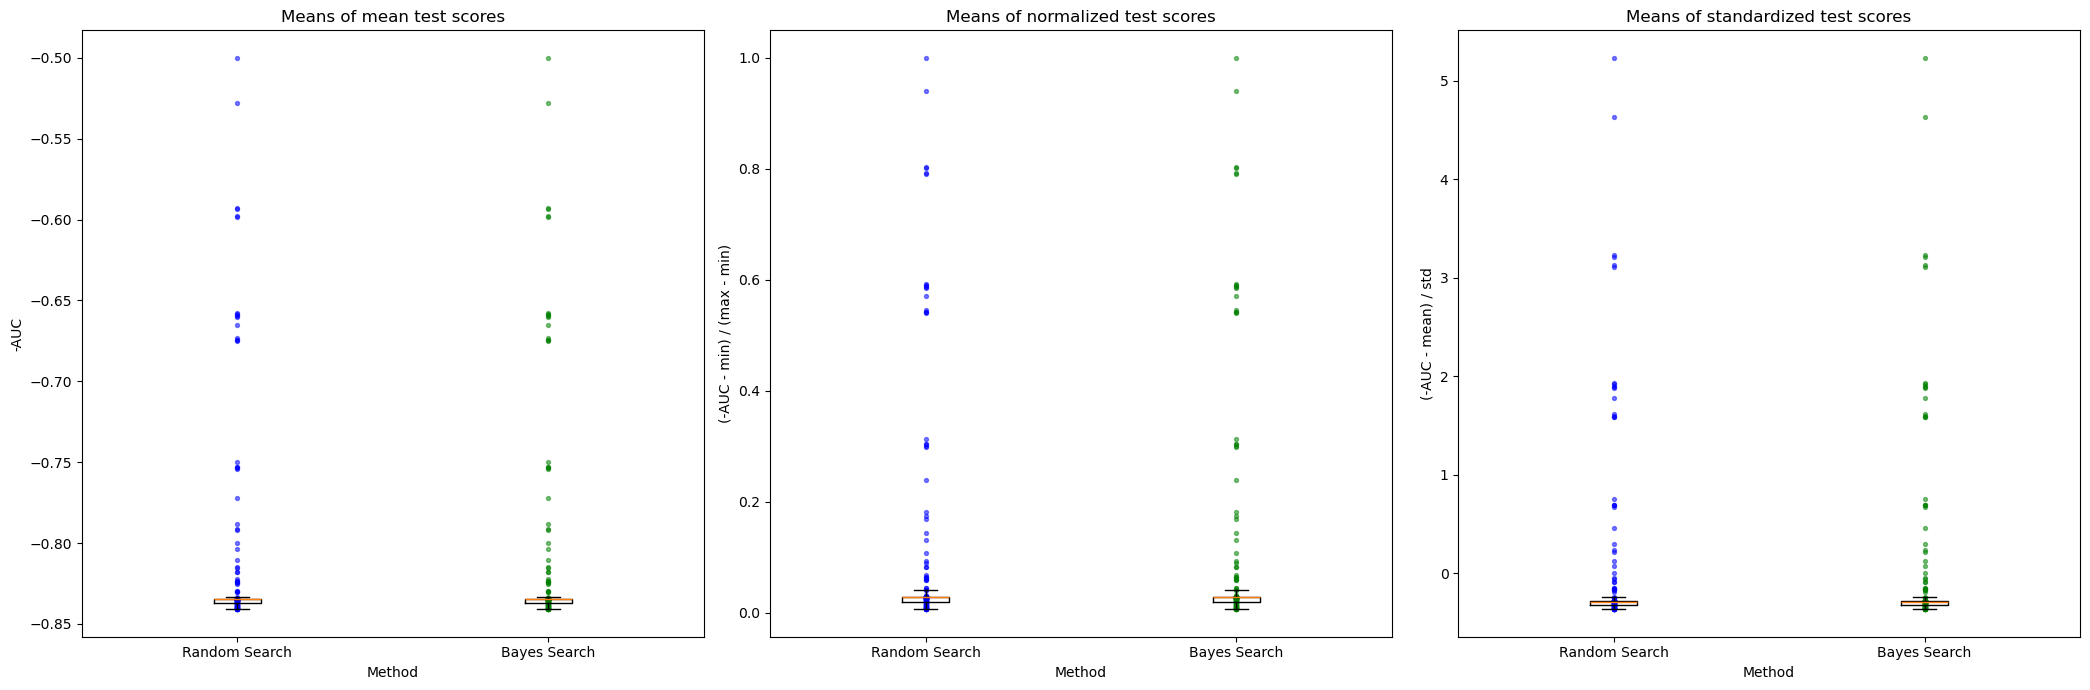
\includegraphics[width=\textwidth]{images/elnet/auc.png}
    \vspace{1ex}
    \caption{Uśrednione po zbiorach danych wartości $R^{(j)}(\theta)$ dla zestawów hiperparametrów. W pierwszym przypadku zastosowanano \textit{-AUC}, w drugim miara została znormalizowana do przedziału [0,1], zaś w trzecim ustandaryzowana. Jak widać różnice w rozkładach nie są duże, zwłaszcza między pierwszym a drugim podejściem.}
    \label{fig:elnet:auc}
\end{figure}
\begin{figure}[H]
    \centering
    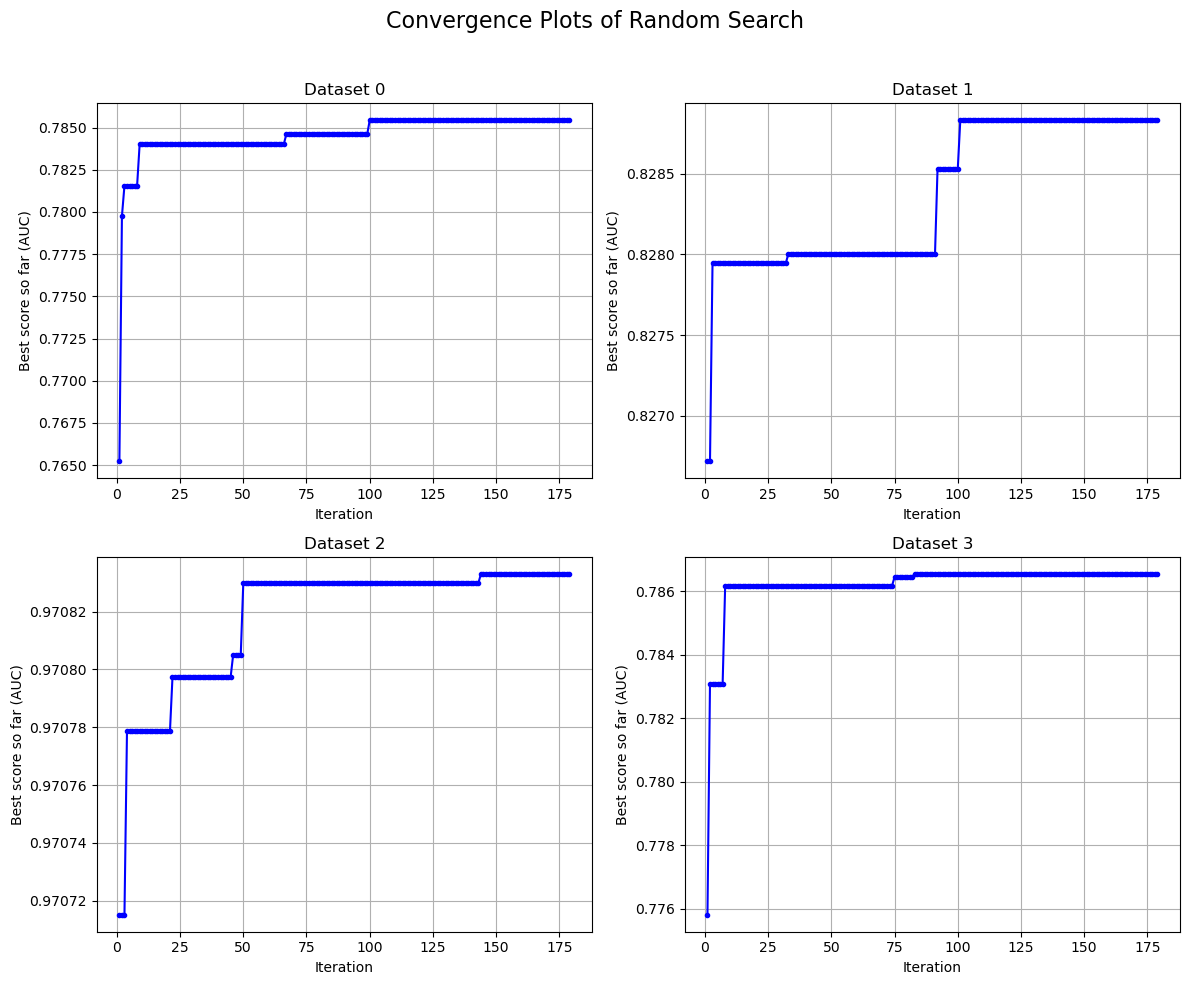
\includegraphics[width=0.9\textwidth]{images/elnet/random_cov.png}
    \vspace{1ex}
    \caption{Wykresy zbieżności metody \textit{Random Search} podczas tunowania algorytmu dla zbiorów danych opisanych w rozdziale \ref{sec:data}. Jak widać już dla 100 iteracji w większości przypadków osiągana jest zbieżność, co jest niewielką liczbą biorąc pod uwagę szybkość metody.}
    \label{fig:elnet:rs}
\end{figure}
\begin{figure}[H]
    \centering
    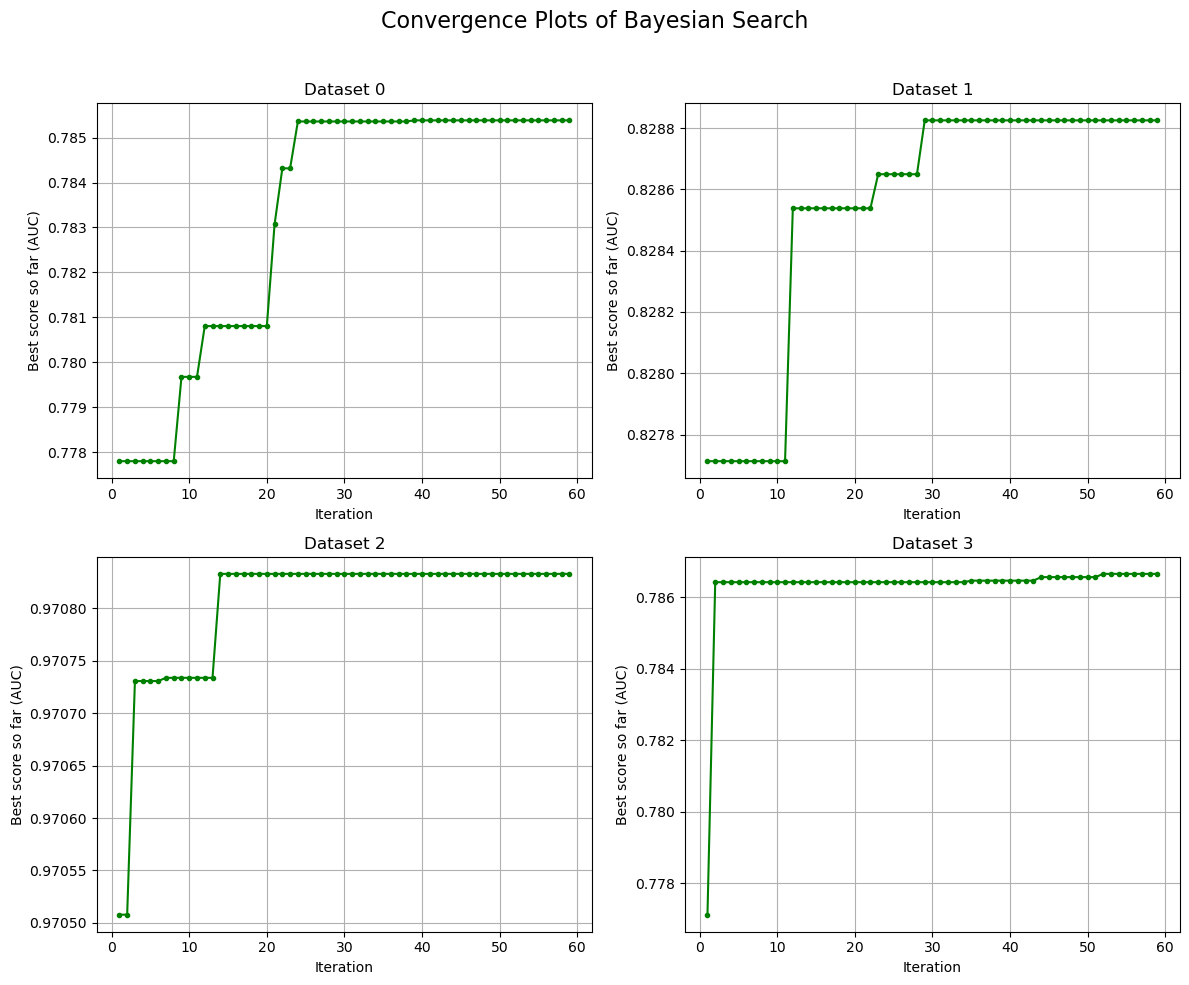
\includegraphics[width=0.9\textwidth]{images/elnet/bayes_cov.png}
    \vspace{1ex}
    \caption{Wykresy zbieżności metody \textit{Bayes Optimization} podczas tunowania algorytmu dla zbiorów danych opisanych w rozdziale \ref{sec:data}. Jak widać metoda potrafi bardzo szybko osiągnąć zbieżność jeżeli wcześnie napotka ekstremum, jednak bezpieczną liczbą iteracji wydaje się być liczba 30.}
    \label{fig:elnet:bo}
\end{figure}
\begin{figure}[H]
    \centering
    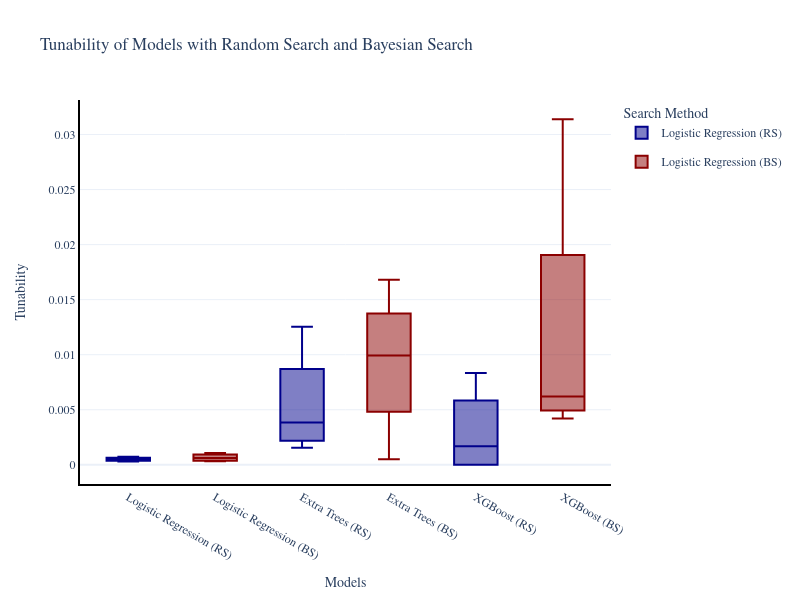
\includegraphics[width=\textwidth]{images/elnet/tunability.png}
    \vspace{1ex}
    \caption{Średnia tunowalność algorytmu \eqref{alg_tun} obliczona dla zestawów hiperparametrów przeszukiwanych podczas jego tunowania. Niezależnie od zestawu optymalnego (którego wpływ widać jedynie poprzez nieznaczne przesunięcie wykresów na osi Y) można dostrzec istotną różnicę pomiędzy rozkładami dla metod \textit{samplingu}.}
    \label{fig:elnet:tun}
\end{figure}
\begin{figure}[H]
    \centering
    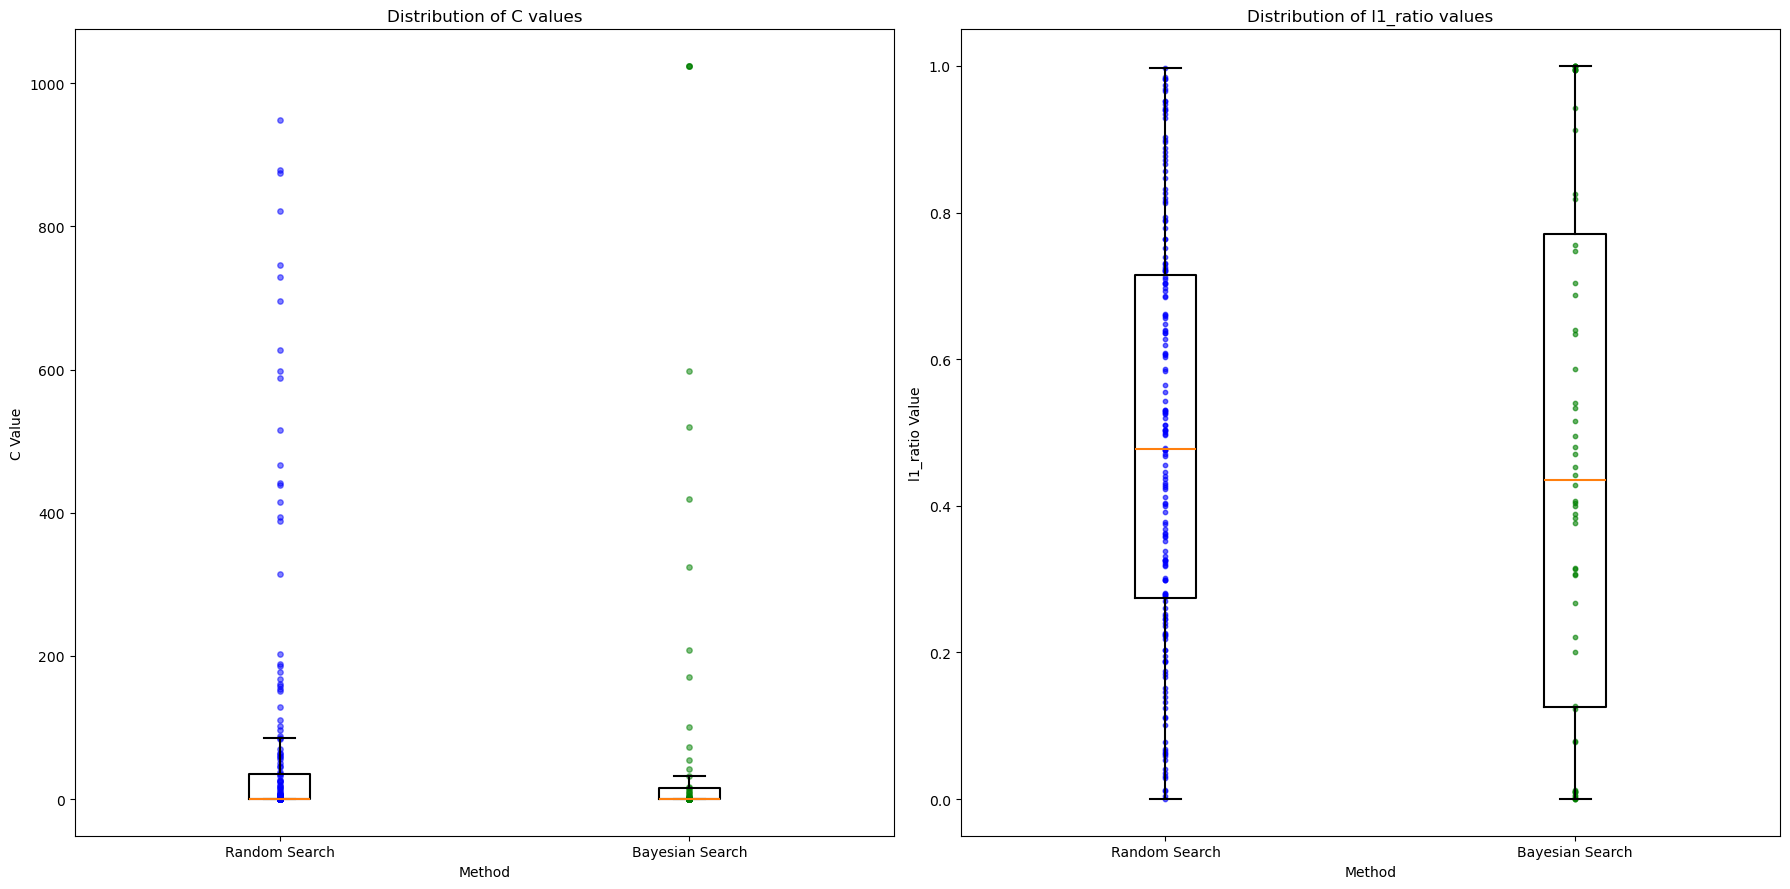
\includegraphics[width=\textwidth]{images/elnet/distribution.png}
    \vspace{1ex}
    \caption{Dystrybucja przeszukiwanych wartości hiperparametrów podczas tunowania algorytmu dla każdej z metod \textit{samplingu}. Jak widać różnice pomiędzy rozkładami według metod są nieduże, jednak same rozkłady hiperparametrów mocno różnią się między sobą, co najpradopodobniej wynika z ich zakresów przyjętych w rozdziale \ref{sec:elnet}.}
    \label{fig:elnet:dist}
\end{figure}

\begin{figure}[H]
    \centering
    \includegraphics[width=0.9\textwidth]{images/xgboost/diabetes_bayes.png}
    \vspace{1ex}
    \caption{Zbieżność dla optymalizaji bayesowskiej dla \textit{XGBoost}, dane \textbf{diabetes}.}
    \label{fig:xg:bayes}
\end{figure}

\begin{figure}[H]
    \centering
    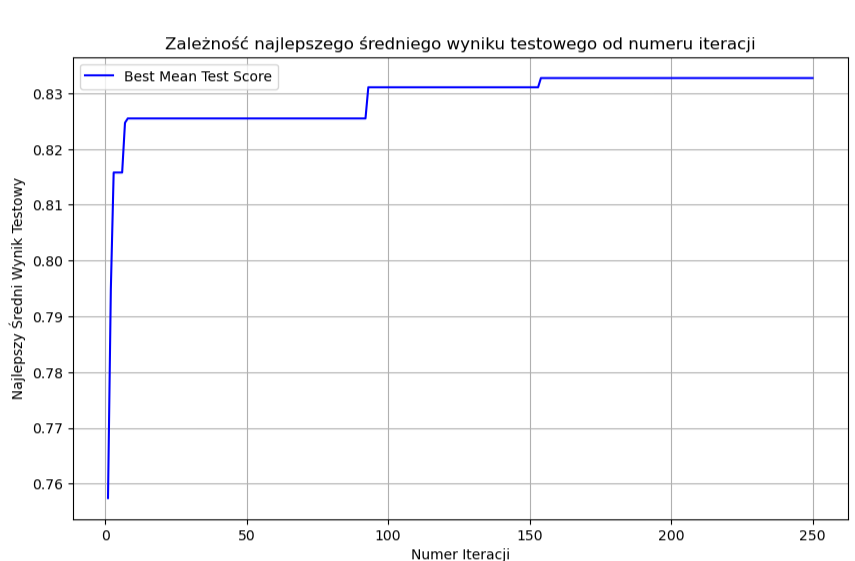
\includegraphics[width=0.9\textwidth]{images/xgboost/diabetes_random.png}
    \vspace{1ex}
    \caption{Zbieżność dla przeszukiwania losowego dla \textit{XGBoost}, dane \textbf{diabetes}.}
    \label{fig:xg:random}
\end{figure}

\begin{figure}[H]
    \centering
    \includegraphics[width=0.9\textwidth]{images/xgboost/diabetes_bayes.png}
    \vspace{1ex}
    \caption{Zbieżność dla optymalizacji bayesowskiej na \textit{XGBoost}, dane \textbf{diabetes}.}
    \label{fig:xg:bayes}
\end{figure}


\begin{figure}[H]
    \centering
    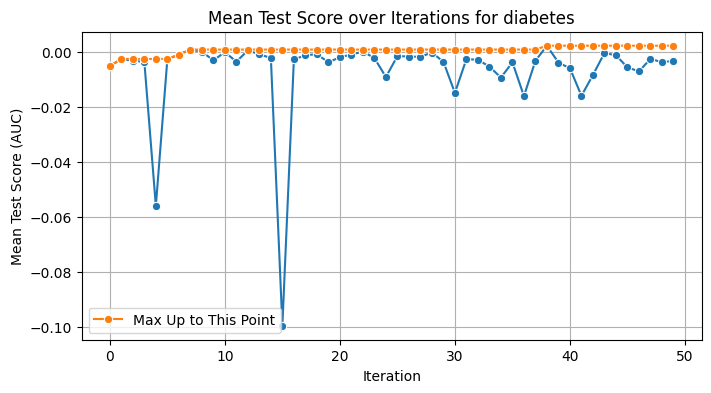
\includegraphics[width=0.9\textwidth]{images/randomforest/diabetes.png}
    \vspace{1ex}
    \caption{Zbieżność dla metody \textit{Random Search} przy użyciu \texttt{RandomForestClassifier}, dane \textbf{diabetes}.}
    \label{fig:xg:random}
\end{figure}

\begin{figure}[H]
    \centering
    \includegraphics[width=0.9\textwidth]{images/randomforest/diabetes_bayes.png}
    \vspace{1ex}
    \caption{Zbieżność dla metody \textit{Bayes Search} przy użyciu \texttt{RandomForestClassifier}, dane \textbf{diabetes}.}
    \label{fig:xg:random}
\end{figure}

\begin{figure}[H]
    \centering
    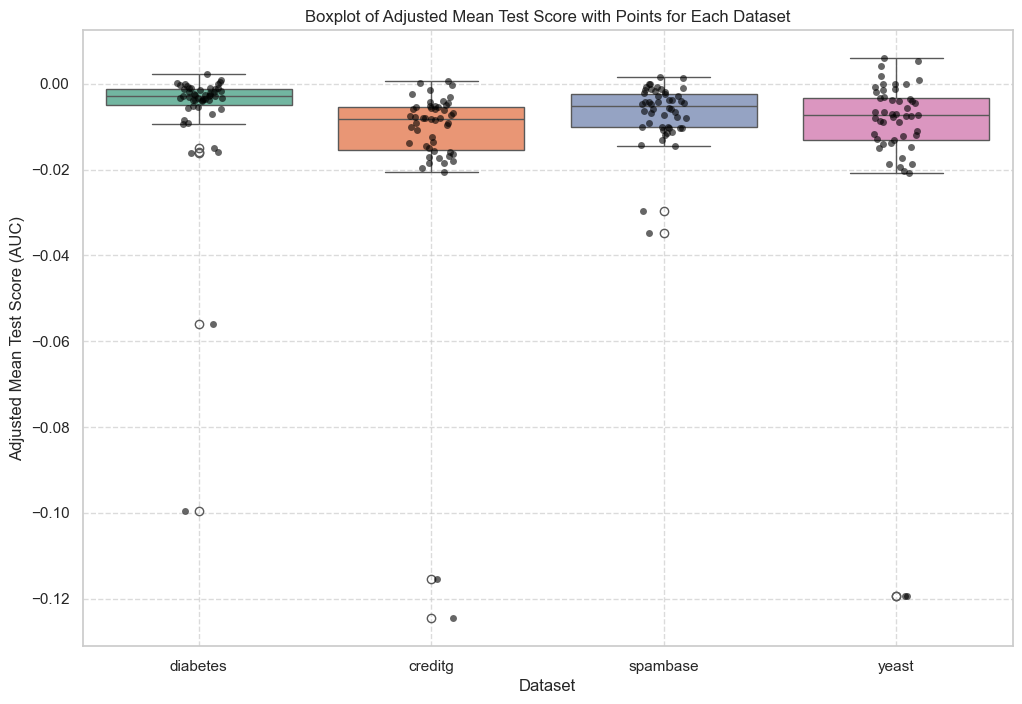
\includegraphics[width=\textwidth]{images/randomforest/boxplot.png}
    \vspace{1ex}
    \caption{Boxplot dla różnych datasetów, metoda \textit{Random Search} dla algorytmu \texttt{RandomForestClassifier}.}
    \label{fig:xg:random}
\end{figure}

\newpage
\bibliographystyle{plain}
\bibliography{refs}
\end{document}
